
\definecolor{cb3b3b3}{RGB}{179,179,179}
\definecolor{cff8080}{RGB}{255,128,128}


\begin{tikzpicture}[y=0.80pt, x=0.8pt,yscale=-1, inner sep=0pt, outer sep=0pt]
\begin{scope}[shift={(0,-782.35975)}]
  \begin{scope}[shift={(0,774.35975)},fill=black]
  \end{scope}
  \path[fill=cb3b3b3] (262.6422,1011.1097) -- (266.1554,1017.1948) --
    (262.7091,1023.1639) -- cycle;
  \path[fill=black] (66.464462,1050.4827) node[above right] (text3075-4-1)
    {Temperature ($T$) [$\,^{o}C$]};
  \path[draw=cb3b3b3,line join=miter,line cap=butt,miter limit=4.00,line
    width=1.600pt] (21.2229,783.8959) -- (21.2229,1017.1368)(263.6121,1017.1368)
    -- (21.2229,1017.1368);
  \path[fill=cb3b3b3] (15.1958,785.7175) -- (21.2809,782.2043) --
    (27.2500,785.6506) -- cycle;
  \path[cm={{0.0,-1.0,1.0,0.0,(0.0,0.0)}},fill=black] (-972.65125,-5.6103458)
    node[above right] (text3075-4-1-6) {\rotatebox{90}{Heat Flux ($\ln
    \left(q^{''}\right)$) [ ]}};
  \path[color=black,fill=cb3b3b3,line width=0.800pt] (63.6562,800.4535) --
    (64.6562,800.4535) -- (64.6562,788.4535) -- (63.6562,788.4535) --
    cycle(63.6562,824.4535) -- (64.6562,824.4535) -- (64.6562,812.4535) --
    (63.6562,812.4535) -- cycle(63.6562,848.4535) -- (64.6562,848.4535) --
    (64.6562,836.4535) -- (63.6562,836.4535) -- cycle(63.6562,872.4535) --
    (64.6562,872.4535) -- (64.6562,860.4535) -- (63.6562,860.4535) --
    cycle(63.6562,896.4535) -- (64.6562,896.4535) -- (64.6562,884.4535) --
    (63.6562,884.4535) -- cycle(63.6562,920.4535) -- (64.6562,920.4535) --
    (64.6562,908.4535) -- (63.6562,908.4535) -- cycle(63.6562,944.4535) --
    (64.6562,944.4535) -- (64.6562,932.4535) -- (63.6562,932.4535) --
    cycle(63.6562,968.4535) -- (64.6562,968.4535) -- (64.6562,956.4535) --
    (63.6562,956.4535) -- cycle(63.6562,992.4535) -- (64.6562,992.4535) --
    (64.6562,980.4535) -- (63.6562,980.4535) -- cycle(63.6562,1016.4535) --
    (64.6562,1016.4535) -- (64.6562,1004.4535) -- (63.6562,1004.4535) -- cycle;
  \path[color=black,fill=cb3b3b3,line width=0.800pt] (123.0625,800.4375) --
    (124.0625,800.4375) -- (124.0625,788.4375) -- (123.0625,788.4375) --
    cycle(123.0625,824.4375) -- (124.0625,824.4375) -- (124.0625,812.4375) --
    (123.0625,812.4375) -- cycle(123.0625,848.4375) -- (124.0625,848.4375) --
    (124.0625,836.4375) -- (123.0625,836.4375) -- cycle(123.0625,872.4375) --
    (124.0625,872.4375) -- (124.0625,860.4375) -- (123.0625,860.4375) --
    cycle(123.0625,896.4375) -- (124.0625,896.4375) -- (124.0625,884.4375) --
    (123.0625,884.4375) -- cycle(123.0625,920.4375) -- (124.0625,920.4375) --
    (124.0625,908.4375) -- (123.0625,908.4375) -- cycle(123.0625,944.4375) --
    (124.0625,944.4375) -- (124.0625,932.4375) -- (123.0625,932.4375) --
    cycle(123.0625,968.4375) -- (124.0625,968.4375) -- (124.0625,956.4375) --
    (123.0625,956.4375) -- cycle(123.0625,992.4375) -- (124.0625,992.4375) --
    (124.0625,980.4375) -- (123.0625,980.4375) -- cycle(123.0625,1016.4375) --
    (124.0625,1016.4375) -- (124.0625,1004.4375) -- (123.0625,1004.4375) -- cycle;
  \path[color=black,fill=cb3b3b3,line width=0.800pt] (198.8125,800.4375) --
    (199.8125,800.4375) -- (199.8125,788.4375) -- (198.8125,788.4375) --
    cycle(198.8125,824.4375) -- (199.8125,824.4375) -- (199.8125,812.4375) --
    (198.8125,812.4375) -- cycle(198.8125,848.4375) -- (199.8125,848.4375) --
    (199.8125,836.4375) -- (198.8125,836.4375) -- cycle(198.8125,872.4375) --
    (199.8125,872.4375) -- (199.8125,860.4375) -- (198.8125,860.4375) --
    cycle(198.8125,896.4375) -- (199.8125,896.4375) -- (199.8125,884.4375) --
    (198.8125,884.4375) -- cycle(198.8125,920.4375) -- (199.8125,920.4375) --
    (199.8125,908.4375) -- (198.8125,908.4375) -- cycle(198.8125,944.4375) --
    (199.8125,944.4375) -- (199.8125,932.4375) -- (198.8125,932.4375) --
    cycle(198.8125,968.4375) -- (199.8125,968.4375) -- (199.8125,956.4375) --
    (198.8125,956.4375) -- cycle(198.8125,992.4375) -- (199.8125,992.4375) --
    (199.8125,980.4375) -- (198.8125,980.4375) -- cycle(198.8125,1016.4375) --
    (199.8125,1016.4375) -- (199.8125,1004.4375) -- (198.8125,1004.4375) -- cycle;
  \path[color=black,fill=cb3b3b3,line width=0.800pt] (91.5938,800.4375) --
    (92.5938,800.4375) -- (92.5938,788.4375) -- (91.5938,788.4375) --
    cycle(91.5938,824.4375) -- (92.5938,824.4375) -- (92.5938,812.4375) --
    (91.5938,812.4375) -- cycle(91.5938,848.4375) -- (92.5938,848.4375) --
    (92.5938,836.4375) -- (91.5938,836.4375) -- cycle(91.5938,862.8954) --
    (92.5938,861.4474) -- (92.5938,860.4375) -- (91.5938,860.4375) -- cycle;
  \path[draw=cff8080,line join=miter,line cap=butt,line width=0.800pt]
    (21.6832,1016.7360) .. controls (41.6832,1001.2904) and (58.4158,990.0033) ..
    (65.6436,961.4885) .. controls (76.2376,908.8152) and (99.9010,814.8548) ..
    (123.2673,815.9439) .. controls (150.3960,816.3400) and (146.3366,895.1518) ..
    (167.2277,919.6073);
  \path[draw=cff8080,dash pattern=on 4.80pt off 1.60pt,line join=miter,line
    cap=butt,miter limit=4.00,line width=0.800pt] (166.9044,919.2232) .. controls
    (180.8648,935.1638) and (189.2079,953.5677) .. (200.4950,953.1716);
  \path[draw=cff8080,line join=miter,line cap=butt,line width=0.800pt]
    (200.3248,953.1934) .. controls (237.1324,951.3126) and (254.1584,857.7261) ..
    (264.0594,801.0924);
  \path[cm={{0.0,-1.0,1.0,0.0,(0.0,0.0)}},fill=black] (-944.72919,37.780823)
    node[above right] (text3075-4-1-6-2) {\rotatebox{90}{subcooled boiling}};
  \path[cm={{0.0,-1.0,1.0,0.0,(0.0,0.0)}},fill=black] (-859.87634,73.486214)
    node[above right] (text3075-4-1-6-3) {\rotatebox{90}{local}};
  \path[cm={{0.0,-1.0,1.0,0.0,(0.0,0.0)}},fill=black] (-817.44995,104.99097)
    node[above right] (text3075-4-1-6-6) {\rotatebox{90}{bulk}};
  \path[fill=black] (130.05948,809.63855) node[above right] (text3075-4-1-0)
    {partial film};
  \path[fill=black] (212.81197,824.7608) node[above right] (text3075-4-1-7) {full
    film};
  \path[fill=black] (75.805504,953.30017) node[above right] (text3075-4-1-0-0)
    {$\substack{\text{nucleate}\\ \text{boiling}}$};
  \path[fill=black] (69.093346,1009.4069) node[above right] (text3075-4-1-0-0-7)
    {$\left(T_{c}-T_{sat}\right)_{JL}=\frac{60\left(\nicefrac{q^{''}}{10^{6}}\right)^{\nicefrac{1}{4}}}{\exp\left(\nicefrac{p}{900}\right)}$};
  \begin{scope}[cm={{0.0,-0.83686,3.7197,0.0,(-155.81765,1270.6028)}},fill=black]
    \path[fill] (356.0799,93.8454) -- (356.0799,95.8962) -- (354.8690,95.8962) ..
      controls (351.6268,95.8962) and (349.4523,95.4144) .. (348.3455,94.4509) ..
      controls (347.2518,93.4873) and (346.7049,91.5667) .. (346.7049,88.6891) --
      (346.7049,83.6501) .. controls (346.7049,81.6970) and (346.3533,80.3428) ..
      (345.6502,79.5876) .. controls (344.9471,78.8324) and (343.6710,78.4548) ..
      (341.8221,78.4548) -- (340.6307,78.4548) -- (340.6307,76.4040) --
      (341.8221,76.4040) .. controls (343.6710,76.4040) and (344.9471,76.0264) ..
      (345.6502,75.2712) .. controls (346.3533,74.5160) and (346.7049,73.1618) ..
      (346.7049,71.2087) -- (346.7049,66.1696) .. controls (346.7049,63.2920) and
      (347.2518,61.3780) .. (348.3455,60.4274) .. controls (349.4523,59.4639) and
      (351.6268,58.9821) .. (354.8690,58.9821) -- (356.0799,58.9821) --
      (356.0799,61.0134) -- (354.7518,61.0134) .. controls (352.9158,61.0134) and
      (351.7179,61.2998) .. (351.1580,61.8727) .. controls (350.5981,62.4457) and
      (350.3182,63.6501) .. (350.3182,65.4860) -- (350.3182,71.0915) .. controls
      (350.3182,73.1488) and (349.9926,74.6201) .. (349.3416,75.5055) .. controls
      (348.6906,76.3910) and (347.5187,77.0290) .. (345.8260,77.4196) .. controls
      (347.5447,77.8623) and (348.7231,78.5199) .. (349.3612,79.3923) .. controls
      (349.9992,80.2647) and (350.3182,81.7230) .. (350.3182,83.7673) --
      (350.3182,89.3727) .. controls (350.3182,91.2087) and (350.5981,92.4131) ..
      (351.1580,92.9860) .. controls (351.7179,93.5589) and (352.9158,93.8454) ..
      (354.7518,93.8454) -- (356.0799,93.8454);
  \end{scope}
  \path[fill=black] (80.098885,1032.9591) node[above right] (text3075-4-1-0-0-7-3)
    {$T_{LB}=T_{sat}+\left(T_{c}-T_{sat}\right)_{JL}-\frac{q^{''}}{h}$};
  \path[color=black,fill=cb3b3b3,line width=0.800pt] (91.5938,1018.1368) --
    (92.5938,1018.1368) -- (92.5938,1006.1368) -- (91.5938,1006.1368) -- cycle;
\end{scope}

\end{tikzpicture}
